


\frame{
  \frametitle{The Importance of Units}


  \begin{minipage}{0.4\linewidth}
    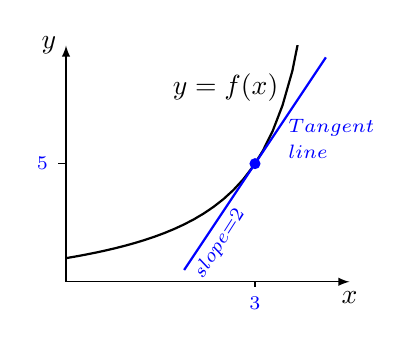
\begin{tikzpicture}[x=12mm,y=6mm,>=latex]
      \draw[black,->] (0,0) -- (3,0) node[below] {$x$};
      \draw[black,->] (0,0) -- (0,5) node[left] {$y$};
      % Ticks:
      \draw[thin,black] (2,0) -- (2,-2pt) node[below,blue] {$\scriptstyle3$};
      \draw[thin,black] (0,2.5) -- (-3pt,2.5) node[left,blue] {$\scriptstyle5$};
      \begin{scope}
        \clip (0,0) rectangle (3,5);
        \draw[black,thick] plot[domain=0:2.5] (\x,{-0.5-3/(\x-3)});
      \end{scope}
      \node[left] at (2.35,{-0.5-3/(2.35-3)}) {$y=f(x)$}; 
      \fill[blue] (2,{-0.5-3/(2-3)}) circle (2pt);
      % Tangent line to y=-0.5-3/(x-3), so y'=3/(x-3)^2 = 3 at x=2.
      % so through (2,2.5) with slope 3; y=3x-3.5
      \draw[thick,blue] (1.25,0.25) -- (2.75,4.75);
      \node[rotate=57.5,blue] at ({1.5+1*0.125},{1-1.5*0.125}) {$\scriptstyle\text{slope}=2$};
      \node[right,blue] at (2.25,3.25) {$\scriptstyle\text{Tangent}$};
      \node[right,blue] at (2.25,2.75) {$\scriptstyle\text{line}$};
    \end{tikzpicture}
  \end{minipage}
  \hfill
  \begin{minipage}{60mm}
    Told $f({\blue 3}) = 5$ and $f{\green '}({\blue 3})={\green 2}$
    \gap

    This means the slope of the tangent line to the graph $y=f(x)$ at $x=3$ is $2$.
    \gap 

    The derivative is this slope, so\ldots
    \gap 

    \fbox{The {\blue units}\ of $\dfrac{dy}{dx}$\ are $\dfrac{\text{units of y}}{\text{units of x}}$}
  \end{minipage}
  \bigskip
  \pause

  \alert{Examples:}

  Heating: derivative units are $\$/{}^{\circ}\ \text{F} = \text{dollars per degree F}$

  Adrenaline: $\text{bpm}/\text{mg} = \text{beats per minute per mg of adrenaline}$.
  \gap

  Units help you understand the {\blue meaning} of the derivative.

}



\frame{
  \frametitle{Interpretation of Derivatives I}

  Suppose $f({\red x})=$ the {\blue percentage of children who still
    get measles} when ${\red x}\%$ of children are inoculated. 
  \gap 

  \alert{Question:}\ Which of the following is a plausible value for $f'(40)$?
  \begin{center}
    A$=0$
    \quad 
    B$= 2$
    \quad 
    C$ = 50$
    \quad 
    D$= -2$
    \quad 
    E$ = -50$
    \pause
    \quad 
    \fbox{D} 
  \end{center}
  \pause
  \gap 

  \alert{Question:}\ If $f({\red 40})={\blue 20}$ and $f'({\red
    40})=-2$, which must be true?
  \begin{itemize}
  \item[A] when 20\% of children are inoculated the  percentage who
    gets measles decreases by $2$\%

  \item[B] when 20\% of children are inoculated then inoculating an
    extra 1\% of children would reduce the number of measles cases by
    another 2\%

  \item[C] If the inoculation rate is 41\% then 18\% of children gets
    measles

  \item[D] If the inoculation rate is 20\% then 2\% fewer cases of
    measles arise if an extra 1\% of children can be inoculated

  \item[E] none of the above
  \pause
  \hfill\alert{Answer:}\ \fbox{C}

  \end{itemize}
}


\frame{
  \frametitle{Interpretation of Derivatives II}

  Air temperature gets colder the higher you go.\\
  $T({\red x})=$ {\blue air temperature} in $^{\circ}C$ at a height $\red x$ meters above sea level.

  \alert{Question:}\ Which of these is a plausible value for $T'({\red 2000})$?
  \begin{center}
    A$ = -1$
    \quad 
    B$ = 1$
    \quad 
    C$ = 0$
    \quad 
    D$ = 1/200$
    \quad 
    E$ = -1/200$
    \pause
    \quad
    \fbox{E} 
  \end{center}
  \pause
  \gap 

  \alert{Question:}\ If $T({\red 2000})={\purple 10}$ and $T{\red'}({\red 2000})=-{\bluegreen 1/200}$, which is most plausible?
  \begin{itemize}
  \item[A] the temperature at sea level is $16^oC$
  \item[B] the temperature $2400$ meters above sea level is $8^oC$
  \item[C] the temperature $10$ meters above sea level is $2000^oC$
  \item[D] 2000 meters above sea level the temperature is decreasing at a rate of $1/200^oC$ per minute.
  \item[E] none of these are plausible
  \end{itemize}
  \pause
  \alert{Answer:}\ \fbox{B}


}



\frame{
  \frametitle{Interpretation of Derivatives III}
  \vspace*{-0.30in}

  \begin{align*}
    {\red x} 
    & = \text{money spent (in thousands of \$) in one month on advertising.}\\
    {\blue f(x)}
    & = \text{{\blue sales} (in thousands of \$) in a month when ${\red x}$ is spent on advertising.}
  \end{align*}
  \pause\vspace*{-0.2in}

  \alert{Question:}\ If $f({\red 20})={\blue 60}$ and $f{\red'}({\red 20})=3$ which must be true?
  \begin{itemize}
  \item[A] When the sales of the company are 20 thousand dollars in
    one month the amount spent on advertising is increasing at a rate
    of 3 thousand dollars per month

  \item[B] When the company spends 20 thousand dollars per month on
    advertising the sales rise at a rate of 3 thousand dollars per
    month 
  \item[C] When the company spends 20 thousand dollars per month on
    advertising each extra dollar a month spent on advertising
    generates an extra 3 dollars of sales. 

  \item[D] When the company spends 3 thousand dollars per month on
    advertising the sales are increasing at a rate of 20 thousand
    dollars per month 

  \item[E] None of the above
    \pause
    \hfill
    \alert{Answer:}\ \fbox{C}
  \end{itemize}

}


